\message{ !name(mainfile.tex)}\documentclass[a4,danish]{article}
\documentclass[11pt,a4paper,twoside,openany,final]{memoir}
\usepackage[utf8]{inputenc}
\usepackage[twoside]{geometry}
%\usepackage[T1]{fontenc}
\usepackage[english]{babel}
\usepackage{amsmath}
\usepackage{amsfonts}
\usepackage{amsthm}
\usepackage[usenames,dvipsnames]{xcolor}
\usepackage{tikz}
\usepackage{amssymb}
\usepackage{graphicx}
\usepackage{flexisym}
\usepackage{hyperref}
\usepackage{xr}
\usepackage[all]{xy}
\usepackage{tikz-cd}
\usepackage{tkz-graph} % To make graphs
\usetikzlibrary{arrows}
\usepackage{tkz-tab}
\usepackage{hyperref}
\usepackage[style=authoryear,backend=bibtex,natbib]{biblatex}
\usepackage{filecontents}
\usepackage[english, status=draft]{fixme}
\fxusetheme{color}
\usepackage{cleveref} 
\usepackage[backgroundcolor=cyan]{todonotes}
\usepackage{wallpaper}
\usepackage{faktor}
\usepackage{nicefrac}
%\usepackage{txfonts}
\usepackage{afterpage} %Til at kunne indsætte tomme sider
\usepackage{pgfplots} %Til at kunne lave grafer
\usepackage{emptypage} %Fjerner sidetal og sidehoveder på tomme sider
\usepackage{multirow}
\usepackage{listings} % To use R language
\lstset{literate=%
{æ}{{\ae}}1
{å}{{\aa}}1
{ø}{{\o}}1
{Æ}{{\AE}}1
{Å}{{\AA}}1
{Ø}{{\O}}1
}
\lstset{ 
  language=R,                     % the language of the code
  basicstyle=\footnotesize\ttfamily, % the size of the fonts that are used for the code
  numberstyle=\tiny\color{blue},  % the style that is used for the line-numbers
  stepnumber=1,                   % the step between two line-numbers. If it is 1, each linewill be numbered
  numbersep=5pt,                  % how far the line-numbers are from the code
  backgroundcolor=\color{white},  % choose the background color. You must add \usepackage{color}
  showspaces=false,               % show spaces adding particular underscores
  showstringspaces=false,         % underline spaces within strings
  showtabs=false,                 % show tabs within strings adding particular underscores
%  frame=single,                   % adds a frame around the code
  rulecolor=\color{black},        % if not set, the frame-color may be changed on line-breaks within not-black text (e.g. commens (green here))
  tabsize=2,                      % sets default tabsize to 2 spaces
  captionpos=b,                   % sets the caption-position to bottom
  breaklines=true,                % sets automatic line breaking
  breakatwhitespace=false,        % sets if automatic breaks should only happen at whitespace
  keywordstyle=\color{RoyalBlue},      % keyword style
  commentstyle=\color{ForestGreen},   % comment style
  xleftmargin=0.5cm,
  xrightmargin=0.5cm
}


%\DisemulatePackage{setspace} START ALTERNATIV SPACING + MARGIN %
%\usepackage{setspace} %
%\doublespacing %
%\setlrmarginsandblock{5cm}{3cm}{*}
%\setulmarginsandblock{2.5cm}{2.5cm}{*}
%\checkandfixthelayout SLUT ALTERNATIV SPACING + MARGIN

\pgfplotsset{width=10cm,compat=1.9}

\begin{filecontents}{bibtest.bib}
@book{Clarke,
  title={Functional Analysis, Calculus of Variations and Optimal Control},
  author={Francis Clarke},
  volume={1},
  year={2013},
  publisher={Springer-Verlag London}
}
@book{Hansen,
  title={Measure Theory},
  author={Ernst Hansen},
  volume={4},
  year={2009},
  publisher={Department of Mathematical Sciences, University of Copenhagen}
}
@article{Topsoee,
  title={Compactness in spaces of measures},
  author={Flemming Topsøe},
  journal={Studia Mathematica},
  volume={36},
  number={3},
  year={1970},
  pages={195--212}
}
@book{Topsoee2,
  title={Topology and measure},
  author={Flemming Topsøe},
  volume={1},
  year={1970},
  publisher={Springer-Verlag, Berlin}
}
@article{Strassen,
  title={The existence of probability measures with given marginals},
  author={Strassen, Volker},
  journal={The Annals of Mathematical Statistics},
  volume={36},
  number={2},
  year={1965},
  pages={423--439}
}
@book{Hoffmann,
  title={Probability in Banach space},
  author={Jørgen Hoffmann-Jørgensen},
  volume={},
  year={1977},
  publisher={Springer}
}
@book{Rudin,
  title={Real and complex analysis},
  author={Walter Rudin},
  volume={3},
  year={1987},
  publisher={McGraw-Hill, Inc.}
}
@book{Rudin2,
  title={Functional analysis},
  author={Walter Rudin},
  volume={2},
  year={1991},
  publisher={McGraw-Hill, Inc.}
}
@book{Aliprantis,
  title={Infinite Dimensional Analysis: A Hitchhiker's Guide},
  author={Charalambos D. Aliprantis and Kim C. Border},
  volume={3},
  year={2006},
  publisher={Springer-Verlag Berlin}
}
@article{Lindvall,
  title={On Strassen's Theorem on stochastic domination},
  author={Torgny Lindvall},
  journal={Electronic Communications in Probability},
  volume={4},
  number={7},
  year={1999},
  pages={51--59}
}
@book{Billingsley,
  title={Convergence of Probability Measures},
  author={Patrick Billingsley},
  volume={2},
  year={2013},
  publisher={John Wiley and Sons}
}
@article{Kamae,
  title={Stochastic inequalities on partially ordered spaces},
  author={Teturo Kamae and Ulrich Krengel and George L. O'Brien},
  journal={The Annals of Probability},
  volume={5},
  number={6},
  year={1977},
  pages={899--912}
}
@book{Sokol,
  title={Advanced Probability},
  author={Alexander Sokol and Anders Rønn-Nielsen},
  volume={4},
  year={2016},
  publisher={Department of Mathematical Sciences, University of Copenhagen}
}
@book{Bladt,
  title={Matrix–exponential distributions in Applied Probability},
  author={Mogens Bladt and Bo Friis Nielsen},
  volume={1},
  year={2017},
  publisher={Springer (Pending)}
}
@article{Rosenblum,
  title={Simple Examples of Estimating Causal Effects Using Targeted Maximum Likelihood Estimation},
  author={Michael Rosenblum and Mark J. van der Laan},
  journal={U.C. Berkeley Division of Biostatistics Working Paper Series},
  volume={Working Paper 262},
  year={2010}
}
@Inbook{Kennedy,
author="Kennedy, Edward H.",
editor="He, Hua
and Wu, Pan
and Chen, Ding-Geng (Din)",
title="Semiparametric Theory and Empirical Processes in Causal Inference",
bookTitle="Statistical Causal Inferences and Their Applications in Public Health Research",
year="2016",
publisher="Springer International Publishing",
address="Cham",
pages="141--167",
isbn="978-3-319-41259-7",
doi="10.1007/978-3-319-41259-7_8",
url="https://doi.org/10.1007/978-3-319-41259-7_8"
}
@book{TargetedLearning,
  title={Targeted Learning in Data Science},
  author={Mark J. van der Laan and Sherri Rose},
  volume={1},
  year={2011},
  publisher={Springer}
}
@article{Wikkelsoee,
  title={Prediction of postpartum blood transfusion -- risk factors and recurrence.},
  author={AJ Wikkelsøe and S Hjortøe and TA Gerds and AM Møller and J Langhoff-Roos}, 
  journal={The journal of maternal-fetal and neonatal medicine},
  volume={27},
  number={16},
  year={2014}
}
@book{Causality,
  title={Elements of causal inference},
  author={Jonas Peters and Dominik Janzing and Bernhard Schölkopf},
  volume={1},
  year={2017},
  publisher={MIT Press}
}
@book{Asymptotic,
  title={Asymptotic Statistics},
  author={A. W. Van der Vaart},
  volume={3},
  year={2000},
  publisher={Cambridge University Press}
}
@article{PPHcause,
  title={Recent Advances in the Management of Major Postpartum Haemorrhage - A Review},
  author={P Reddi Rani1 and Jasmina Begum}, 
  journal={Journal of Clinical and Diagnostic Research},
  volume={11},
  number={2},
  year={2017}
}
@Manual{SuperLearner,
    title = {SuperLearner: Super Learner Prediction},
    author = {Eric Polley and Erin LeDell and Chris Kennedy and Mark {van der Laan}},
    year = {2018},
    note = {R package version 2.0-23},
    url = {https://CRAN.R-project.org/package=SuperLearner}
}
@Article{tmle,
    title = {{tmle}: An {R} Package for  Targeted Maximum Likelihood Estimation},
    author = {Susan Gruber and Mark J. {van der Laan}},
    journal = {Journal of Statistical Software},
    year = {2012},
    volume = {51},
    number = {13},
    pages = {1--35},
    url = {http://www.jstatsoft.org/v51/i13/},
}



\end{filecontents}

\addbibresource{bibtest.bib}


\chapterstyle{verville}


\setlength{\parindent}{0em}
\setlength{\parskip}{1em}
\renewcommand{\baselinestretch}{1}


\DeclareMathOperator{\supp}{supp}
\DeclareMathOperator{\Ext}{Ext}
\DeclareMathOperator{\Aut}{Aut}
\DeclareMathOperator{\Ran}{Ran}
\DeclareMathOperator{\Prob}{Prob}
\DeclareMathOperator{\conv}{conv}
\DeclareMathOperator{\AR}{AR}
\DeclareMathOperator{\Homeo}{Homeo}

\makepagestyle{abs}
    \makeevenhead{abs}{}{}{}
    \makeoddhead{abs}{}{}{}
    \makeevenfoot{abs}{}{\scshape I }{}
    \makeoddfoot{abs}{}{\scshape  I }{}
    %\makeheadrule{abs}{\textwidth}{\normalrulethickness}
    %\makefootrule{abs}{\textwidth}{\normalrulethickness}{\footruleskip}
\pagestyle{abs}


\makepagestyle{cont}
    \makeevenhead{cont}{}{}{}
    \makeoddhead{cont}{}{}{}
    \makeevenfoot{cont}{}{\scshape II }{}
    \makeoddfoot{cont}{}{\scshape  II }{}
    %\makeheadrule{abs}{\textwidth}{\normalrulethickness}
    %\makefootrule{abs}{\textwidth}{\normalrulethickness}{\footruleskip}
\pagestyle{cont}

\newcommand{\lv}{\lVert}
\newcommand{\rv}{\rVert}


\renewcommand\chaptermarksn[1]{}
\nouppercaseheads
\createmark{chapter}{left}{shownumber}{}{.\space}
\makepagestyle{dut}
    \makeevenhead{dut}{\scshape\rightmark}{}{}
    \makeoddhead{dut}{\scshape\leftmark}{}{}
    \makeevenfoot{dut}{}{\scshape $-$ \thepage\ $-$}{}
    \makeoddfoot{dut}{}{\scshape $-$ \thepage\ $-$}{}
    \makeheadrule{dut}{\textwidth}{\normalrulethickness}
    \makefootrule{dut}{\textwidth}{\normalrulethickness}{\footruleskip}
\pagestyle{dut}

\makepagestyle{chap}
    \makeevenhead{chap}{}{}{}
    \makeoddhead{chap}{}{}{}
    \makeevenfoot{chap}{}{\scshape $-$ \thepage\ $-$}{}
    \makeoddfoot{chap}{}{\scshape $-$ \thepage\ $-$}{}
    \makefootrule{chap}{\textwidth}{\normalrulethickness}{\footruleskip}
\copypagestyle{plain}{chap}

\newcommand{\R}{\mathbb{R}}
\newcommand{\C}{\mathbb{C}}
\newcommand{\N}{\mathbb{N}}
\newcommand{\E}{\mathrm{E}}
\newcommand{\Var}{\mathrm{Var}}
\newcommand{\mbr}{(X,\mathcal{A})}
\newcommand{\Z}{\mathbb{Z}}
\newcommand{\Q}{\mathbb{Q}}
\newcommand{\F}{\mathcal{F}}
\newcommand{\A}{\mathcal{A}}
\newcommand{\cc}{C_c}
\newcommand{\PP}{\mathcal{P}}
\newcommand{\B}{\mathcal{B}}
\newcommand{\ee}{\epsilon}
\newcommand{\la}{\lambda}
\renewcommand{\H}{\mathcal{H}}
\newcommand{\pp}{\text{Prob}}
\newcommand{\U}{\mathcal{U}}
\newcommand{\dd}{\mathrm{d}}

\newcommand{\nocontentsline}[3]{}
\newcommand{\tocless}[2]{\bgroup\let\addcontentsline=\nocontentsline#1{#2}\egroup} % Fjern sections fra Table of Contents

\makeatletter
\newcommand{\Spvek}[2][r]{%
  \gdef\@VORNE{1}
  \left(\hskip-\arraycolsep%
    \begin{array}{#1}\vekSp@lten{#2}\end{array}%
  \hskip-\arraycolsep\right)}

\def\vekSp@lten#1{\xvekSp@lten#1;vekL@stLine;}
\def\vekL@stLine{vekL@stLine}
\def\xvekSp@lten#1;{\def\temp{#1}%
  \ifx\temp\vekL@stLine
  \else
    \ifnum\@VORNE=1\gdef\@VORNE{0}
    \else\@arraycr\fi%
    #1%
    \expandafter\xvekSp@lten
  \fi}
\makeatother

\def\acts{\curvearrowright}

\newcommand{\K}{\mathbb{K}}

\newtheoremstyle{break}
	{\topsep}{\topsep}
	{\bfseries}{}
	{\newline}{}
\theoremstyle{break}
\newtheorem{theorem}[subsection]{Theorem}
\newtheorem{lemma}[subsection]{Lemma}
\newtheorem{proposition}[subsection]{Proposition}
\newtheorem{corollary}[subsection]{Corollary}
\newtheorem{definition}[subsection]{Definition}
\newtheoremstyle{Break}
	{\topsep}{\topsep}
	{}{}
	{\bfseries}{}
	{\newline}{}
\theoremstyle{Break}
\newtheorem{example}[subsection]{Example}
\newtheorem{remark}[subsection]{Remark}
\newtheorem{note}[subsection]{Note}
\setcounter{secnumdepth}{0}
\usepackage{xpatch}
\xpatchcmd{\proof}{\ignorespaces}{\mbox{}\\\ignorespaces}{}{}

\newcommand*{\diff}{\mathop{}\!\mathrm{d}}

\newcommand\blankpage{%
    \null
    \thispagestyle{empty}%
    \addtocounter{page}{-1}%
    \newpage}
    
\DeclareNameAlias{sortname}{last-first} % Med flere forfattere bliver alle navne på formen
\DeclareNameAlias{default}{last-first} % : "LastName, FirstName MiddleName

\newcommand{\blank}{\makebox[1ex]{\textbf{$\cdot$}}} % Command to placeholder

\newcommand{\indep}{\rotatebox[origin=c]{90}{$\models$}} % Independent symbol

\title{Statistical analysis of shapes}
\author{Mads and Anders}
\date{\today}

%%% Local Variables:
%%% mode: latex
%%% TeX-master: "mainfile"
%%% End:


\begin{document}

\message{ !name(L2-metric.tex) !offset(-7) }
\subsection{The L2 metric vanishes}
\label{sec:l2-metric-vanishes}

In the previous section we went through some work to construct a measure of length for a path $q$ in the space $\mathcal{I}$. As the tangent spaces were seen to consist of some functions on the circle, it was natural to consider using a version of the L$^2$-metric (a version invariant to reparametrizations). However, as we illustrate in this section, this does not give rise to a usable notation of length, because the geodesic distance following from this metric becomes 0 for every two curves in the space.

It can seem weird to go through so much trouble to define a useless distance. But firstly, the construction illustrates some of the difficulties in defining a reasonable notion on length on $\mathcal{I}$; secondly, and more importantly, the fact that the distance vanishes is a quite surprising result, which depends crucially on the formula for the length of a path given in Proposition~\ref{prop:length-quotient}. This gives us some justification for the somewhat unfruitfull work of definiting the L$^2$-metric.

The ``proof'' below is mostly heuristic, and we only consider the very simply case of a path transforming the circle into a larger circle, but this captures the main idea.
\begin{theorem}
  \label{theorem:l2-metric-vanishes}
  For all $\mathrm{a},\mathrm{b} \in \mathcal{I}$
  \begin{equation*}
    \mathcal{D}(\mathrm{a},\mathrm{b}) = 0.
  \end{equation*}
\end{theorem}

\begin{proof}[Proof of Theorem~\ref{theorem:l2-metric-vanishes}]

  \begin{figure}
    \centerline{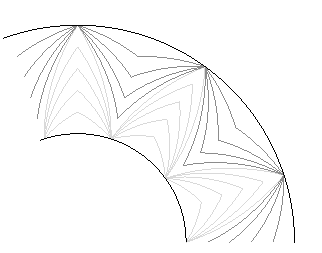
\includegraphics[width=0.6\linewidth]{zigzag-path0.pdf}}
    \caption[]{Illustration of a zigzag path moving the unit circle to the circle with radius 2. The path first moves the points along the path sketched in light-gray and then moves them along the dark-gray path.}
    \label{fig:zigzag-path}
  \end{figure}

  By the definition of the length $\mathcal{D}$ we need to show that for any two paths $\mathrm{a},\mathrm{b} \in \mathcal{I}$ and any $\epsilon >0 $ there exists a path $\mathrm{q}$ in $\mathcal{I}$ such that
  \begin{equation*}
    \mathcal{L}(\mathrm{q}) < \epsilon.
  \end{equation*}
  The trick is to construct a path in $\I$ that moves in zigzag and then use Proposition~\ref{prop:length-quotient} to calculate the length of this path in $\mathcal{I}$.
  It turns out that when we increase the number of teeth of the zigzag path, the length of the path decreases in $\mathcal{I}$.
  The idea of such a zigzag path is illustrated in figure~\ref{fig:zigzag-path}.

  To see why this  pheonomenon happens, first rewrite the \eqref{eq:length-quotient} from Proposition~\ref{prop:length-quotient} as
  \begin{align*}
    \mathcal{L}(q) &
                     = \int_{0}^{1}
                     \left(
                     \int_{\S^{1}} \frac{\langle q_{t},i q_{\theta}\rangle^2}
                     {|q_{\theta}|}  \diff \theta
                     \right)^{1/2} \diff t \\
                   & =  \int_{0}^{1}
                     \left(
                     \int_{\S^{1}}
                     \left(
                     \frac{\langle q_{t},i
                     q_{\theta}\rangle}{| q_{t}|| q_{\theta}|}
                     \right)^2
                     | q_t|^2   | q_{\theta}|
                     \diff \theta
                     \right)^{1/2} \diff t \\
                   &  =
                     \int_{0}^{1}
                     \left(
                     \int_{\S^{1}}
                     \cos(\alpha( q_t, i q_{\theta}))^2
                     | q_t|^2   | q_{\theta}|
                     \diff \theta
                     \right)^{1/2}\diff t,
  \end{align*}
  with $\alpha(x,y)$ denoting the angle between $x$ and $y$.
  When constructing a zigzag-path the angle will for large enough $n$ be given approximately by
  \begin{equation}
    \label{eq:tan-angle}
    2n \approx \tan(\alpha).
  \end{equation}
  Note that this does not depend on $\theta$ nor $t$.
  \hl{[Maybe not completely obvious that this holds.]}
  See figure~\ref{fig:angle-arg} for a visual justification of this.
  \begin{figure}[h]
    \centering
    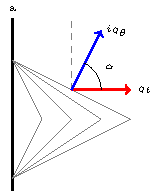
\includegraphics[width=0.5\linewidth]{angle-argument.pdf}
    \caption{Relative to $q_t$, $iq_{\theta}$ is by construction a line with slope $2n$, and thus the angle between these two vectors are found by \eqref{eq:tan-angle}. Note that the starting curve, $\mathrm{a}$, is here represented as a straight line to simplify the calculations; this should be a reasonable approximation when $n$ is large.}
    \label{fig:angle-arg}
  \end{figure}

  We have that
  \begin{equation*}
    \cos(\arctan(2n)) = (1+(2n)^2)^{-1/2}
    = O(n^{-1}),
  \end{equation*}
  so we can write
  \begin{equation}
    \label{eq:approx-L-angle}
    \begin{aligned}
    \mathcal{L}( \mathrm{q} )
    & =
      \int_{0}^{1}
      \left(
      \int_{\S^{1}}
      O(n^{-1})^2
      | q _t|^2   | q _{\theta}|
      \diff \theta
      \right)^{1/2} \diff t \\
    & =
      O(n^{-1})
      \int_{0}^{1}
      \left(
      \int_{\S^{1}}
      | q _t|^2   | q _{\theta}|
      \diff \theta
      \right)^{1/2} \diff t.
    \end{aligned}
  \end{equation}
  To show that our zigzag path has arbitrary small length we thus just need to show that the remaining integral does not grow faster than $n^{2}$. Figure~\ref{fig:zigzag-path-angle} illustrates how the angle $\alpha$ increases towards $\pi/2$, making $\cos(\alpha) \rightarrow 0$; at the same time, it is seen how $q_{\theta}$ grows -- not fast enough, however, to kill the $\cos(\alpha)$ term, it turns out.

\begin{figure}
  \centering
  \begin{subfigure}{.49\textwidth}
    \centering
    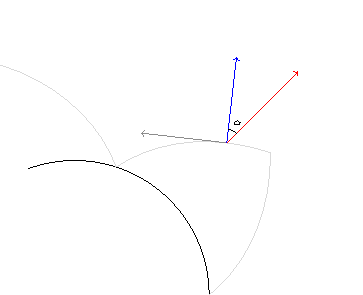
\includegraphics[width=1\linewidth]{zigzag-path.pdf}
  \end{subfigure}
  \begin{subfigure}{.49\textwidth}
    \centering
    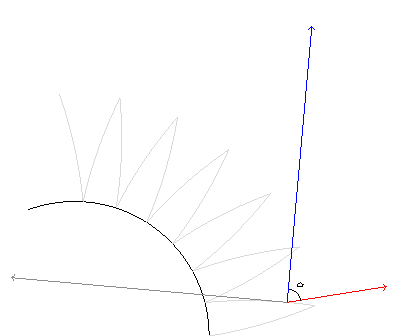
\includegraphics[width=1\linewidth]{zigzag-path2.pdf}
  \end{subfigure}
  \caption{Illustration of how the angle $\alpha$ increases with the number of teeth of the zigzag path. The red vector gives the time derivate, the gray the path derivative, and the blue the normal of the path derivative. The zigzag path is shown in light-gray in the background. (Note that the length of the vectors are scaled to fit the drawing and does not necessarily reflect an exact relationship between the lengths of the two.)}
  \label{fig:zigzag-path-angle}
\end{figure}

As an example, we take the simply case where we expand the circle $e^{i\pi\theta}$ to
$2e^{i\pi\theta}$. The zigzag path in then concretely given as
\begin{equation*}
  \phi(t,\theta) = e^{i\pi\theta}
  \sum_{k=0}^{n-1}
  h^{n,k}(t,\theta) + g^{n,k}(t,\theta)
\end{equation*}
where
\begin{equation*}
  \begin{aligned}
    h^{n,k}(t,\theta) & := 1_{[\frac{k}{n},\frac{k}{n} +
      \frac{1}{2n})}(\theta) \left( 1+2t(n\theta-k) \right), \\
    g^{n,k}(t,\theta) & := 1_{[\frac{k}{n} + \frac{1}{2n},\frac{k+1}{n})}(\theta)
    \left( 1+2t(1-n\theta-k) \right).
  \end{aligned}
\end{equation*}
We have that
\begin{equation*}
  \begin{aligned}
    |\phi_t| & = \sum_{k=0}^{n-1} |h^{n,k}_t| + \sum_{k=0}^{n-1}
    |g^{n,k}_t|, \\
    |\phi_{\theta}| & = \sum_{k=0}^{n-1} |h^{n,k}_{\theta} + h^{n,k} | +
    \sum_{k=0}^{n-1}
    |g^{n,k}_{\theta} + g^{n,k} |,
  \end{aligned}
\end{equation*}
so by symmetry
\begin{equation*}
  \begin{aligned}
    \int_{0}^{1}
    |\phi_t|^2   |\phi_{\theta}|
    \diff \theta
    & =
    2n \int_{0}^{\frac{1}{2n}} |h^{n,0}_t|^2 |h^{n,0}_{\theta} + h^{n,0} |
    \diff \theta \\
    & = 2n \int_{0}^{\frac{1}{2n}}
    (2n\theta)^2(2tn+1+t2n\theta) \diff \theta \\
    & = \int_{0}^1
    u^2(2tn+1+t u) \diff \theta \\
    & = O(n),
  \end{aligned}
\end{equation*}
for $t\in[0,1]$. Plugging this into \eqref{eq:approx-L-angle} gives the result.
\end{proof}




%%% Local Variables:
%%% mode: latex
%%% TeX-master: "mainfile"
%%% End:

\message{ !name(mainfile.tex) !offset(-171) }

\end{document}
